% Short paper (workshop length). Scientific source: ../manuscript.md v0.8 and the
% tracked result records it cites. Build: latexmk -pdf -interaction=nonstopmode
% -halt-on-error -outdir=output main.tex
\documentclass[10pt,letterpaper]{article}
\usepackage[T1]{fontenc}
\usepackage[utf8]{inputenc}
\usepackage{lmodern}
\usepackage[margin=1in]{geometry}
\usepackage{microtype,amsmath,amssymb}
\usepackage{graphicx,booktabs,array,caption}
\usepackage[numbers,sort&compress]{natbib}
\usepackage{xurl}
\usepackage[dvipsnames]{xcolor}
\usepackage[colorlinks=true,linkcolor=MidnightBlue,citecolor=MidnightBlue,urlcolor=MidnightBlue]{hyperref}
\captionsetup{font=small,labelfont=bf}
\setlength{\tabcolsep}{4pt}
\newcommand{\lam}{\lambda}
\hypersetup{pdftitle={Learned Deferral Did Not Beat Confidence in a Same-Model Thinking Cascade}}

\title{Learned Deferral Did Not Beat Confidence\\in a Same-Model Thinking Cascade}
\author{Anonymous authors}
\date{}

\begin{document}
\maketitle

\begin{abstract}
Hybrid reasoning models such as Qwen3 can answer directly or think first, so a cheap policy is to draft an answer directly and pay for a thinking solve only when the draft looks unreliable. We ask whether a learned deferral rule chooses those escalations better than the standard baseline, a threshold on the draft's token-level confidence, when the utility charges for both calls. On 50 GSM8K questions with eight independent draws per mode, Qwen3-1.7B's thinking solve fixes 30 of 400 direct drafts and breaks 10. Yet neither a predeclared learned rule, nor nine follow-up rules (stronger regularization, contrastive objectives, released contrastive-language-model heads, and token-level uncertainty), nor a simulated two-draft agreement rule improves on confidence for held-out questions. The predeclared learner has lower utility than confidence at every cost preference we tested; once refitting variation is included, its interval includes zero, so it fails to beat confidence without being reliably worse. Confidence itself captures 17.6\% of the gain of a hindsight oracle, which no deployable rule can match. For Qwen3-0.6B, deferral beats random escalation at equal cost by 6.2 accuracy points, but most of its utility gain over accepting the draft comes from thinking itself; for Qwen3-1.7B, confidence deferral does not pay. The panels are small and were reused across analyses; we report every predeclared criterion, including those that failed.
\end{abstract}

\section{Introduction}

Hybrid reasoning models such as Qwen3 \citep{qwen2025qwen3} offer a direct mode and a thinking mode in one set of weights. Thinking is usually more accurate but costs several times as many output tokens. A natural policy is to answer directly first and to think only when the direct draft looks unreliable. In the language of model cascades, the direct mode is the first stage, the thinking mode is the second, and a deferral rule decides when to call the second stage \citep{chen2023frugalgpt,jitkrittum2023cascade}. Unlike most language-model cascades, both stages here are the same model.

Prior work on cascades gives a reason to expect a simple confidence rule to be hard to beat. \citet{jitkrittum2023cascade} characterize the optimal deferral rule and show that confidence is highly competitive on many regular classification tasks. Learned post-hoc rules can significantly improve on it when the second model is a specialist, when labels are noisy, or when the distribution shifts, but may offer little when the second model's outputs are hard to predict. \citet{gupta2024lmcascades} find that sequence-level uncertainty in generative cascades is length-biased and that learned deferral on token-level uncertainty quantiles helps. For deciding when to reason, \citet{lewislim2026confidencegated} find that training-free confidence measures can reduce redundant reasoning but are inconsistent: for some models, including Qwen3-8B, no measure consistently beats random gating, and GSM8K shows limited benefit.

We test whether learned post-hoc deferral improves on confidence in this same-model cascade, under a fixed contract. A small Qwen3 model first writes a direct draft. A rule then accepts the draft or requests a fresh thinking solve of the same question; the thinking call does not see the draft. Because the draft is already paid for, escalation charges both calls. We collect eight independent responses per mode for each of 50 GSM8K questions \citep{cobbe2021gsm8k}, fit rules on some questions, and evaluate them on others. The setting is deliberately small, like a deployment calibrated on a small labelled set: each fold trains on 40 questions, and the 30 rescues come from only 11 of the 50 questions. Section~\ref{sec:results} shows that even the draft features alone, which include confidence, do not help.

Our findings are as follows.
\begin{itemize}
\item \textbf{Observed opportunities did not become better deferral.} Thinking rescues 30 of 400 drafts (a wrong draft followed by a correct thinking solve), yet the predeclared learner fails four of its five success criteria on held-out questions, and nine follow-up rules and a two-draft agreement rule also fail to improve on confidence (Table~\ref{tab:main}).
\item \textbf{The comparison is not specific to one cost.} Refitted at ten cost preferences, the predeclared learner has lower utility than confidence at every one, and most learned rules lie below random escalation at equal cost (Figure~\ref{fig:curves}).
\item \textbf{The gap is a missing gain, not a demonstrated loss.} For the predeclared learner, intervals that hold fitted actions fixed exclude zero, but intervals that include refitting variation do not (Table~\ref{tab:refit}).
\item \textbf{Whether deferral pays depends on the solver.} For Qwen3-0.6B, confidence deferral beats random escalation by 6.2 points at equal cost, and its gain over accepting the draft stays positive with refitting, though most of that gain comes from thinking itself. For Qwen3-1.7B it does not pay. Lower confidence is associated with higher gain only for the smaller model.
\end{itemize}
None of the ingredients is new: confidence-gated thinking \citep{lewislim2026confidencegated}, post-hoc deferral after an observed draft \citep{jitkrittum2023cascade,gupta2024lmcascades}, agreement-based routing \citep{yue2024motcascade,lee2026dart}, and learned routers (Section~\ref{sec:related}) all precede this work. Our contribution is a controlled test of learned deferral in the case where both stages are the same small hybrid model, with repeated draws per question, held-out questions, a utility that charges the draft, intervals that include refitting variation, and every predeclared criterion reported. The answer is negative: confidence was not beaten, which fits the caveats in the cascade analysis about when post-hoc rules may not help, and the larger practical lever was whether thinking pays for the solver at all.

\section{Setup}
\label{sec:setup}

\paragraph{Decision and utility.} Let $D$ be a completed direct response and $T$ a fresh thinking response, with scored correctness $Y_D,Y_T\in\{0,1\}$ and charged output tokens $C_D,C_T$ (including inserted closure tokens). Action $a=1$ requests thinking and $a=0$ accepts the draft. The utility and the gain from deferring are
\begin{equation}
U(a)=Y_D+a(Y_T-Y_D)-\lam(C_D+aC_T)/1000,\qquad G=Y_T-Y_D-\lam C_T/1000,
\end{equation}
with $\lam=0.05$ fixed before the studies. Utility is measured in correct answers per question: a difference of $+0.01$ is one more correct answer per 100 questions, and $\lam=0.05$ prices 20,000 output tokens at one correct answer. Because $U$ is linear in $a$, a rule that knew $\mathbb{E}[G\mid x,D]$ would defer exactly when it is positive, which parallels the optimal deferral rule of \citet{jitkrittum2023cascade}. A confidence rule defers when the draft's mean token log probability, computed after the sampling transformations (temperature, top-$k$, top-$p$), falls below a threshold chosen on training questions only. It can approach the optimal rule only if lower confidence means higher expected gain, an analogue of their Lemma 4.1. A learned post-hoc rule instead estimates $G$ from permitted features: the question and the observed draft, but never the thinking output, its length, or the reference answer.

\paragraph{Data and solvers.} All questions are GSM8K training rows assigned to frozen roles; the official test split stays sealed. The main panel (50 questions, eight draws per mode) uses Qwen3-1.7B with 2,048 reasoning tokens and 512 answer tokens, sampled with the recommended settings. A separate two-solver panel (64 other questions) runs Qwen3-0.6B and Qwen3-1.7B with two draws per mode and solver. Correctness comes from a frozen numeric answer scorer (numeric-v7); rejected or truncated outputs count as wrong, and no human scoring audit was performed. Reference answers were opened only after each study's full set of responses was complete.

\paragraph{Evaluation.} Each main-panel question has eight independently seeded responses per mode. Pairing the direct and thinking responses with the same draw index gives 400 draft--thinking pairs, which we call states. Five outer folds of ten questions keep every evaluation question out of fitting and tuning. A rule is fitted on draws 0--3 of the 40 training questions and evaluated on draws 4--7 of the 10 held-out questions, and vice versa; we report the average of the two directions. Four inner question folds choose settings. Intervals use 2,000 whole-question bootstrap resamples (90\%) with fitted actions held fixed, unless stated otherwise.

\paragraph{Rules.} The predeclared learner is Ridge regression of $G$ on 387 question features (MiniLM sentence embeddings \citep{reimers2019sbert,wang2020minilm,sentencetransformersAllMiniLML6v2} and three lexical counts) and four draft features (confidence, log length, parser validity, truncation); it defers when predicted gain is positive. Its comparator is the best of accept, escalate, and confidence, chosen within training. Later bounded studies, each with its own frozen grid and success criterion, tested stronger regularization and compression, compact contrastive and cross-entropy objectives, released contrastive-language-model (CLM) heads \citep{kwok2026clm,contrastiveLM2026release} with a matched-encoder control, token-level uncertainty quantiles adapted from \citet{gupta2024lmcascades}, and a two-draft agreement rule adapted from DART \citep{lee2026dart}. Two of these follow-up rules, zero-shot CLM and the minimum-token threshold, involve no learned weights beyond a threshold. Each follow-up rule had to beat confidence by at least $+0.01$ utility, with positive means in both directions and positive leave-one-question-out averages. Appendix~\ref{app:rules} gives the details.

\section{Results}
\label{sec:results}

\subsection{No tested rule beats confidence}

Table~\ref{tab:main} lists the rules on the main panel at $\lam=0.05$. Direct accuracy is 89.5\% and thinking accuracy 94.5\%. Of the 400 paired states, 30 are rescues, 10 are harms, 348 have both responses correct, and 12 have both wrong. The rescues come from 11 of the 50 questions, and rescues or harms from 14.

The predeclared learner's utility difference against its training-selected comparator is $-0.016$ (90\% interval $[-0.033, -0.001]$), and four of its five success criteria fail. Against confidence it is lower by $0.044$. Even its training-selected comparator, which picks accept, escalate, or confidence on the training questions, trails fixed confidence by $0.028$, which shows how noisy selection is with 40 training questions. The same Ridge on the four draft features alone, which include confidence, is also lower ($-0.030$), so the 387 question features do not explain the loss by themselves. Every follow-up rule also has lower point utility than confidence, and every success criterion fails. The closest rules are two-draft agreement ($-0.003$), which escalates only 8.5\% of states, and a threshold on the lowest token log probability ($-0.010$).

\begin{table}[t]
\centering
\caption{Main panel, Qwen3-1.7B, $\lam=0.05$, averaged over both draw directions (400 states). Accuracy and escalated (the share of states sent to thinking) are in percent; tokens per state include the paid draft. Differences are against confidence, with 90\% whole-question intervals holding fitted actions fixed; rows without an interval were not bootstrapped against confidence. Lift is accuracy minus random escalation at the same token cost, in percentage points. $^\dagger$Derived from the reported accuracy and tokens. $^\ddagger$Computed from the rule's recorded decisions.}
\label{tab:main}
\small
\begin{tabular}{@{}lrrrlr@{}}
\toprule
Rule & Accuracy & Tokens & Escalated & Utility vs.\ confidence [90\%] & Lift \\
\midrule
Always direct & 89.50 & 221 & 0.0 & $-0.012$ $[-0.034, +0.007]$ & 0.00 \\
Always think & 94.50 & 1,611 & 100.0 & $-0.032$ & 0.00 \\
Hindsight oracle (not deployable) & 97.00 & 342 & 7.5 & $+0.057$ & $+7.07$ \\
\textbf{Confidence} & \textbf{92.75} & \textbf{628} & \textbf{25.0} & reference & $\mathbf{+1.78}$ \\
\midrule
\multicolumn{6}{@{}l}{\emph{Learned on question and draft features}} \\
Predeclared learner (Ridge) & 89.00 & 757 & 40.5 & $-0.044$ $[-0.064, -0.025]$ & $-2.43$ \\
\quad Its training-selected comparator & 90.25 & 683 & 29.8 & $-0.028^\dagger$ & $-0.91$ \\
\quad Same Ridge, draft features only & 89.75 & 622 & 28.0 & $-0.030^\dagger$ & $-1.19$ \\
\quad Same Ridge, question features only & 88.75 & 794 & 43.0 & $-0.048^\dagger$ & $-2.81$ \\
Stronger-penalty and PCA Ridge variants & 90.75 & 514 & 18.0$^\ddagger$ & $-0.014$ $[-0.026, -0.004]$ & $+0.20$ \\
Compact neural heads (four objectives) & 89.25 & 605 & 26.0$^\ddagger$ & $-0.034$ $[-0.053, -0.017]$ & $-1.63$ \\
\midrule
\multicolumn{6}{@{}l}{\emph{Contrastive-language-model (CLM) features}} \\
Released CLM, zero-shot & 94.75 & 1,551 & 95.0$^\ddagger$ & $-0.026$ $[-0.059, +0.017]$ & $+0.47$ \\
Released CLM, calibrated & 88.50 & 444 & 15.3$^\ddagger$ & $-0.033$ $[-0.054, -0.015]$ & $-1.80$ \\
PCA8 and Ridge on the CLM encoder & 89.00 & 331 & 7.8$^\ddagger$ & $-0.023$ $[-0.044, -0.004]$ & $-0.89$ \\
Best CLM-based rule, chosen in training & 88.75 & 406 & 13.0$^\ddagger$ & $-0.029$ $[-0.050, -0.011]$ & $-1.42$ \\
\midrule
\multicolumn{6}{@{}l}{\emph{Token-level uncertainty}} \\
Learned error score & 88.75 & 570 & 23.3$^\ddagger$ & $-0.037$ $[-0.061, -0.013]$ & $-2.01$ \\
Minimum-token threshold & 91.00 & 483 & 16.3$^\ddagger$ & $-0.010$ $[-0.027, +0.005]$ & $+0.56$ \\
Gain Ridge & 90.00 & 483 & 16.8$^\ddagger$ & $-0.020$ $[-0.035, -0.007]$ & $-0.44$ \\
\midrule
Two-draft agreement (simulated) & 92.25 & 598 & 8.5 & $-0.003$ $[-0.021, +0.012]$ & $+1.40^\dagger$ \\
\bottomrule
\end{tabular}
\end{table}

\subsection{The point ordering holds at every tested cost}

Figure~\ref{fig:curves}A places each rule on accuracy and cost. Random escalation at a fixed rate traces the dashed line between always direct and always think. Confidence lies 1.78 points above that line at $\lam=0.05$, while the predeclared learner lies 2.43 points below it. We refitted the original rules at ten values of $\lam$ from 0 to 0.3. The predeclared learner has lower utility than confidence at all ten (by 0.006 to 0.054) and lower than its training-selected comparator at all ten. Among the follow-up rules, only the minimum-token threshold, zero-shot CLM, and the stronger-penalty Ridge variants lie above the random line, each by less than 0.6 points; two-draft agreement lies 1.40 points above it. The single cost preference of the original studies therefore does not explain the result.

\begin{figure}[t]
\centering
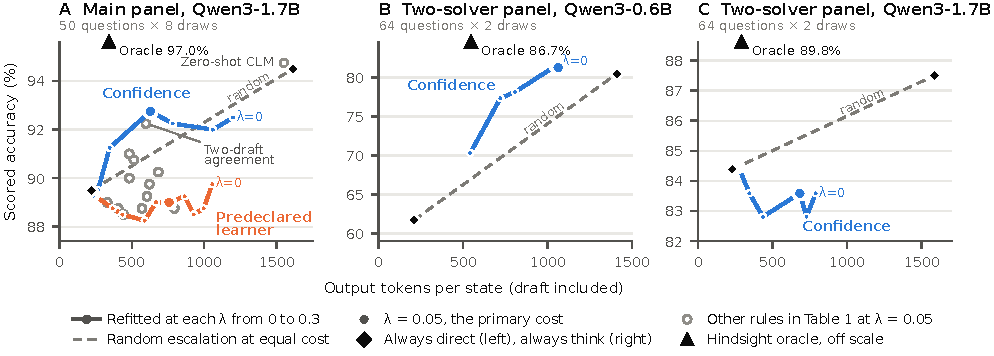
\includegraphics[width=\textwidth]{figures/output-r2/pdf/figure-1-accuracy-cost-r2.pdf}
\caption{Accuracy and output cost of the deferral rules. Lines trace rules refitted at ten cost preferences ($\lam$ from 0 to 0.3; large dots at $\lam=0.05$), and hollow circles are the other rules in Table~\ref{tab:main}. The dashed line is random escalation at equal cost; triangles mark the hindsight oracle, above each axis. Panels use different axes. Values are post-hoc, from reused development panels, and carry no intervals.}
\label{fig:curves}
\end{figure}

\subsection{With refitting, the gap is a missing gain}

Fixed-action intervals treat each fitted rule as given. To include the variation from fitting, we resampled whole questions 2,000 times and refitted the rules on each resample. Each copy of a question kept its original fold, and inner folds were formed over distinct questions, so no question appeared in both training and evaluation. Separately, 200 random repartitions of the questions into folds isolate the effect of fold assignment.

\begin{table}[t]
\centering
\caption{90\% intervals with fitted actions held fixed and with refitting included, for utility contrasts at $\lam=0.05$. Copied questions in the refit bootstrap reduce the number of distinct training questions, so those intervals are approximate. The last column gives the 5th--95th percentiles over 200 fold repartitions.}
\label{tab:refit}
\small
\begin{tabular}{@{}lrlll@{}}
\toprule
Contrast & Point & Fixed actions & With refitting & Fold repartitions \\
\midrule
Learner $-$ training-selected comparator & $-0.016$ & $[-0.033, -0.001]$ & $[-0.042, +0.021]$ & $[-0.036, -0.005]$ \\
Learner $-$ confidence & $-0.044$ & $[-0.064, -0.025]$ & $[-0.058, +0.008]$ & $[-0.051, -0.029]$ \\
Confidence $-$ accept (1.7B, main panel) & $+0.012$ & $[-0.007, +0.034]$ & $[-0.027, +0.028]$ & $[+0.003, +0.015]$ \\
Confidence $-$ accept (0.6B, two-solver) & $+0.153$ & $[+0.086, +0.220]$ & $[+0.068, +0.220]$ & $[+0.131, +0.168]$ \\
Confidence $-$ accept (1.7B, two-solver) & $-0.031$ & $[-0.056, -0.006]$ & $[-0.051, +0.010]$ & $[-0.037, -0.016]$ \\
\bottomrule
\end{tabular}
\end{table}

Refitting widens the intervals by 1.1 to 1.9 times (Table~\ref{tab:refit}). It also pulls the bootstrap means toward zero (for the learner against its comparator, $-0.012$ against the point estimate $-0.016$), so these intervals lean toward including zero. The intervals for the learner's gap to both comparators now include zero, as does the 1.7B confidence loss on the two-solver panel. The fold assignment does not drive the signs: every repartition range stays on the side of its point estimate. We conclude that the predeclared learner did not deliver its predeclared gain of at least $+0.01$; the data do not show that it is worse than confidence. Against confidence, the upper end of its refit interval ($+0.008$) lies below the $+0.01$ margin, so a gain of that size is approximately ruled out; against the training-selected comparator (upper end $+0.021$) it is not. Only this learner and confidence were refitted; the follow-up rules' fixed-action intervals in Table~\ref{tab:main} would also widen if refitting were included.

\subsection{Deferral pays for the smaller solver only}

On the two-solver panel (Figure~\ref{fig:curves}B--C), Qwen3-0.6B's direct accuracy is 61.7\% and its thinking accuracy 80.5\%. Confidence deferral reaches 81.25\% at 1,063 tokens per state, 6.2 points above random escalation at equal cost, and gains $+0.153$ utility over accepting the draft. That gain stays clear of zero with refitting and is positive at every $\lam$ up to 0.2, but most of it is the value of thinking: always thinking after the draft already gains $+0.128$, and confidence leads always thinking by only $+0.025$, a difference without an interval. For Qwen3-1.7B, direct accuracy is 84.4\% and thinking 87.5\%. Confidence deferral is 1.8 points below random escalation at equal cost and has lower utility than accepting the draft at every $\lam$ tested. On the main panel, its gain over accepting the 1.7B draft ($+0.012$) is not distinguishable from zero. The two-draft agreement rule also fails its screen on this panel. It trails confidence by 0.028 for Qwen3-0.6B. For Qwen3-1.7B it leads confidence by 0.008, positive in both draws but below the $+0.01$ margin, yet trails accepting the draft by 0.023.

\section{Why confidence was hard to beat}

\paragraph{Few opportunities, many costly mistakes.} At $\lam=0.05$ the average thinking call costs about 0.07 utility, so more than about one escalation in fourteen must be a rescue before harms are counted. The hindsight oracle escalates exactly the 30 rescues (7.5\% of states) and reaches 97.0\% at 342 tokens. Confidence escalates 100 states: 17 rescues, 4 harms, 4 pairs in which both responses are wrong, and 75 pairs in which both were already correct. It therefore captures 17.6\% of the oracle's gain. The oracle sees the realized thinking response, so part of its gain is sampling luck that no rule using only the question and draft can capture; the share understates confidence relative to any achievable rule. The predeclared learner escalates 162 states but rescues only 4.

\paragraph{Where the rescues sit.} A post-hoc audit grouped states into five confidence bins. For Qwen3-0.6B, mean gain falls at every step from the lowest-confidence bin to the highest, and the two lowest bins hold 23 of 32 rescues: confidence is the right ranking. For Qwen3-1.7B on the main panel, only the lowest-confidence fifth has positive mean gain ($+0.081$, interval $[-0.016, +0.176]$), and 13 of the 30 rescues sit in higher bins, outnumbered by states whose only gain is the thinking cost. The highest-confidence bin holds 8 of the 12 pairs in which both responses are wrong; these drafts are confidently wrong and thinking does not fix them. On the 1.7B two-solver panel, no confidence threshold improves on accepting the draft even in-sample. A learned rule would need features that find the remaining rescues among many already-correct drafts, from 40 training questions per fold and 391 features. None of the tested rules did. Gain does vary between questions (post-hoc between-question variance 0.032, 90\% interval $[0.005, 0.065]$), so the results do not show that deferral is unlearnable, only that these rules did not learn it from 40 training questions.

\paragraph{What cascade analysis does and does not explain.} Confidence traces the same deferral curve as the optimal rule when it orders inputs the same way as the gain from deferring (Lemma 4.1 of \citet{jitkrittum2023cascade}). The bins above suggest that an analogue of this holds roughly for Qwen3-0.6B but not for Qwen3-1.7B, so we have no reason to think confidence is near-optimal on the larger solver, although the hindsight oracle overstates the usable headroom because it sees the realized thinking response. The three settings in which they show post-hoc rules helping are at most partly present. The second stage is the same model and more accurate on average (94.5\% against 89.5\%), but its errors are not uniform: on the 1.7B two-solver panel, 12 of the 18 thinking responses that hit the reasoning cap are wrong, against 4 of the other 110. A rule cannot see a cap hit before paying for thinking, and we did not test directly whether question or draft features predict it. Training and evaluation questions come from the same pool, so there is no designed shift. We injected no label noise. In their label-noise case both models fail on low-confidence inputs, so confidence wastes deferrals on them. The closest analogue here, pairs in which both responses fail, differs by panel: on the main panel 8 of 12 sit in the highest-confidence bin, where a confidence rule does not escalate, but on the 1.7B two-solver panel 10 of 13 sit in the two lowest bins, where it does. They also warn that post-hoc rules may devolve to plain confidence deferral when the second model's outputs are not strongly predictable, and their excess-risk bound has an estimation term that shrinks with the size of the fitting sample. Both caveats fit this setting: the predeclared test that question-level gain is reproducible did not pass, and each fold trains on 40 questions. This reading is consistent with the failures but was not tested directly.

\paragraph{Token-level features added no usable signal.} \citet{gupta2024lmcascades} find that summing token log probabilities over-defers long outputs and that averaging over-corrects toward short ones. Our confidence is the average, and it is nearly uncorrelated with answer length (Spearman $-0.027$). Low token quantiles rank errors slightly better in-sample (positive-gain AUROC 0.761 against 0.705) without improving held-out decisions. On accuracy tasks their rule is a five-layer MLP trained to predict that the large model is right and the small one wrong; with 40 training questions per fold we fitted logistic and Ridge models instead, so ours is not a test of their model class or target.

\paragraph{Agreement is priced out.} Two-draft agreement nearly matches confidence while escalating a third as often. If the second draft were free, it would lead confidence by 0.008; at $\lam=0.05$ its cost, about 0.011 utility per state, removes the advantage. Settings where a second draft is cheap relative to thinking were not tested.

\section{Related work}
\label{sec:related}

\paragraph{Learning to defer and selective prediction.} Our decision descends from learning to defer to an expert \citep{madras2018defer,mozannar2020defer}, including post-hoc estimators fitted after both models are fixed \citep{narasimhan2022posthoc}, and from selective prediction, which abstains when confidence is low \citep{geifman2017selective}. A learned calibrator helps selective question answering under domain shift \citep{kamath2020selective}, one of the settings in which \citet{jitkrittum2023cascade} find that learned rules beat confidence.

\paragraph{Cascades and routing.} Cascades of models of increasing size can improve both efficiency and accuracy \citep{wang2022committees,varshney2022cascading}. For language models, FrugalGPT learns when to continue to a stronger model \citep{chen2023frugalgpt}; \citet{yue2024motcascade} defer on the consistency of sampled answers; AutoMix uses self-verification and a POMDP router \citep{aggarwal2024automix}; \citet{fanconi2025cascaded} place an accept-or-regenerate decision before human escalation; and \citet{dekoninck2024cascaderouting} unify routing and cascading. Routers choose a model before generation \citep{ding2024hybridllm,ong2024routellm} or from confidence tokens trained into the model \citep{chuang2024confidencetokens}. \citet{jitkrittum2023cascade} analyze when confidence-based deferral suffices, and \citet{gupta2024lmcascades} study token-level uncertainty for generative cascades. Our primary learner is close to the Diff-01 post-hoc estimator of \citet{jitkrittum2023cascade}, a squared-error regression on the difference in correctness, with token cost added to the target.

\paragraph{Adaptive thinking.} Reasoning models often spend many tokens on easy problems \citep{chen2024overthinking,sui2025overthinking}, and skipping the thinking phase can outperform thinking at matched token budgets \citep{ma2025nothinking}. Test-time compute can be allocated per prompt by difficulty or predicted benefit \citep{snell2024testtime,damani2024hardtothink}, controlled by budget forcing \citep{muennighoff2025s1}, or decided by the model itself after training with reinforcement learning \citep{jiang2025lhrm,zhang2025adaptthink,fang2025thinkless}. Most of these decide before a draft exists or change the model; our rules see a completed draft and leave the model unchanged. \citet{lewislim2026confidencegated} gate chain of thought on direct-answer confidence, with Qwen3-8B/32B and two GPT models on seven benchmarks including GSM8K. Benefits depend on the dataset and model, which matches our solver dependence, and their perplexity measure is also a transform of a mean token log probability. Their direct mode outputs only a final answer, whereas our direct drafts average 221 tokens, so the settings are not directly comparable. We add learned rules and repeated draws per question, and we charge both calls on every escalation; their released analysis code counts only the reasoning response. DART routes after observing two direct drafts \citep{lee2026dart}; our agreement rule simulates its first stage without budget probing and is not a faithful comparison. Self-Route \citep{he2025selfroute} and BEST-Route \citep{ding2025bestroute} choose modes or sample counts before generation.

\paragraph{Confidence and agreement.} Our confidence is a sequence-level uncertainty score of the kind studied for autoregressive models by \citet{malinin2021structured}. Neural-network confidence is often miscalibrated \citep{guo2017calibration}, but a threshold rule depends only on the ranking. Language models can also judge whether their own answer is true \citep{kadavath2022know}, state a confidence in words \citep{xiong2024express}, or be scored by semantic entropy over samples \citep{kuhn2023semantic}; we tested none of these. Self-consistency votes over sampled answers \citep{wang2023selfconsistency}, and adaptive variants stop sampling once answers agree \citep{aggarwal2023adaptiveconsistency,li2024esc}. Our two-draft agreement rule applies the same idea with two drafts and escalates to thinking when they disagree.

\paragraph{Evaluation.} Variation from data sampling, initialization, and hyperparameter choice markedly affects benchmark comparisons \citep{bouthillier2021variance}, and cross-validation estimates the average error of models fitted on other training sets rather than the error of the fitted model \citep{bates2024crossvalidation}; this is why Table~\ref{tab:refit} includes refitting. Recent audits caution that routing headroom need not be usable value \citep{chen2026routingoracle,garg2026unsolvability}, and that predicting failure differs from predicting which intervention pays \citep{yang2026failureprotocol}. RouterDC \citep{chen2024routerdc}, cost-aware contrastive routing \citep{shirkavand2025cscr}, and SEMIROUTER \citep{wang2026semirouter} precede our use of repeated labels and contrastive representations.

\section{Limitations}

The study uses one dataset on which the larger solver is near ceiling, and two small solvers from one family. The predeclared learner and all follow-up rules reuse the same 50 questions, and later analyses, including the cost curves, refit intervals, confidence bins, token-level rules, and agreement simulation, are post-hoc on those panels. The intervals that include refitting cover five contrasts and are approximate; the other intervals hold fitted actions fixed. Correctness is scorer-based, with no human audit. The token-level and agreement rules are adaptations, not reproductions, and we compare against no external system. We tested no verbalized, self-evaluated, or sampling-based confidence measure, and the thinking call never sees the draft. Our questions come from the GSM8K training split, which may be in Qwen3's training data, and GSM8K scores may overstate reasoning ability \citep{mirzadeh2025gsmsymbolic}. Each fold trains on 40 questions, fewer than nine of which contain a rescue on average. We used one prompt and one decoding configuration, and token counts from the two model sizes are not equal compute. All intervals are 90\% and none is adjusted for multiple comparisons. Earlier development studies on other questions gave mixed results for agreement. Utility counts output tokens only, not input processing, encoder work, or latency. Two later interventions, a parser guard tested on 228 fresh questions and a larger reasoning allowance on 11 selected questions, each produced at most one rescue and no supported gain; the technical report gives details.

\section{Conclusion}

In a same-model cascade from a direct draft to a fresh thinking solve, observed rescues did not become better learned deferral. Confidence had the highest point utility among the deferral rules we tested on the main panel, yet it captured 17.6\% of the hindsight gain, and it paid only for the smaller solver. The settings in which post-hoc rules are known to help were at most partly present, each fold trained on 40 questions, and the predeclared test that question-level gain is reproducible did not pass. Tasks with more rescue opportunities, cheaper second stages, or real distribution shift are where a learned rule would have room to win, and a larger prospective study would be needed to show it.

\paragraph{Declarations.} Author contributions, funding, and conflicts of interest will be supplied by the authors. AI assistance was used for drafting and research support; the authors are responsible for the claims and references.

\paragraph{Code and data availability.} Code, frozen protocols, and a cache of scored outcomes, draft features, and recorded decisions will be released after review. From that cache alone, a check script recomputes the study values in Tables~\ref{tab:main} and~\ref{tab:refit}, every point in Figure~\ref{fig:curves}, and the main quoted values (195 checks, all passing; cache SHA-256 \nolinkurl{3da91b57c98612141f2962cc657d6c9e3e26b4b0592d52006a7dcfce92e73757}). Values added during revision come from the tracked study reports or from a second script over the same cache. GSM8K is released under the MIT license and the Qwen3 models under Apache-2.0; no human subjects or personal data were involved.

\bibliographystyle{unsrtnat}
\bibliography{references}

\appendix
\section{Rules and settings}
\label{app:rules}

\paragraph{Models and generation.} Qwen3-1.7B (revision 70d244cc) and Qwen3-0.6B (revision c1899de2), local float16 inference with batch size one. Direct sampling: temperature 0.7, top-p 0.8, top-k 20. Thinking sampling: temperature 0.6, top-p 0.95, top-k 20. Reasoning allowance 2,048 tokens, answer allowance 512 tokens; forced closure, when needed, is charged. The prompt asks for the numerical answer in \verb|\boxed{}|.

\paragraph{Predeclared learner.} Combined Ridge on 391 features, penalty chosen from $\{1, 10, 100\}$ by inner question folds, with training-only standardization. The comparator is chosen within training from accept, escalate, and a confidence threshold. Training conditions use 1, 2, or 4 draws per training question; the four-draw average across directions is primary, and an eight-draw condition is secondary. The five criteria were a positive reproducibility test of question-level gain, positive gains in both four-draw directions, an average gain of at least $+0.01$ with a positive lower bound, no reversal in the eight-draw condition, and at least ten informative questions; only the last passed.

\paragraph{Follow-up rules.} \emph{CPU family:} Ridge penalties $\{10^2, 10^3, 10^4\}$, PCA compression to eight question components, and conservative confidence corrections, 1,035 Ridge fits in total. \emph{Compact neural:} two representations crossed with four objectives (gain regression, regret-weighted cross-entropy, bidirectional contrastive, binary cross-entropy) on a 120-parameter head, one optimization seed; drafts were encoded from their last 256 tokens, which truncated 111 of 400. \emph{CLM:} released heads on 4-bit Qwen3-8B last-token states, zero-shot and with scalar calibration, plus a PCA8/Ridge control on the same embeddings; these rules use the encoder representation only, without confidence or other draft statistics. \emph{Token-level:} nine quantiles of teacher-forced token log probabilities before the sampling transformations, their mean, and log length; a logistic error score (primary), a minimum-token threshold, and gain Ridge. \emph{Agreement:} each evaluation draft is paired with every other draw in its half; it is accepted if both parse to the same number and escalated otherwise; both drafts are charged. All follow-up rules select settings on training questions and draws only.

\section{Reproducibility}

Every study froze its protocol, grid, endpoints, and criteria before execution and recorded source, input, and output hashes. All generation ran on local hardware and charged about 1.2 million output tokens across the main panel, the two-solver panel, and the two later interventions. No rule passed its predeclared criteria, so the sealed confirmation questions and the official GSM8K test split were never used. Earlier development studies used an older scorer and different questions; they are summarized, with all criteria and records, in an accompanying technical report that will be made available after review.

\end{document}
